% ----------------------------------------------------------
% Apêndices
% ----------------------------------------------------------
\begin{apendicesenv}

% Imprime uma página indicando o início dos apêndices
% \partapendices

% Configuração global de estilo para todos os códigos
\definecolor{codered}{RGB}{221,0,0}
\definecolor{codegreen}{RGB}{0,170,0}
\definecolor{codebrown}{RGB}{146,73,0}
\definecolor{codeorange}{RGB}{255,119,0}
\definecolor{backcolour}{RGB}{255,255,255}

\lstdefinestyle{mystyle}{
    backgroundcolor=\color{backcolour},   
    commentstyle=\color{codered},
    keywordstyle=\color{codeorange},
    numberstyle=\tiny\color{codebrown},
    stringstyle=\color{codegreen},
    basicstyle=\ttfamily\footnotesize,
    breakatwhitespace=false,         
    breaklines=true,                 
    captionpos=b,                    
    keepspaces=true,                 
    numbers=left,                    
    numbersep=5pt,                  
    showspaces=false,                
    showstringspaces=false,
    showtabs=false,                  
    tabsize=2,
    frame=single,
    frameround=tttt,
    rulecolor=\color{black!30},
    aboveskip=20pt,
    belowskip=20pt
}

\lstset{style=mystyle}

% Configuração para acentuação
\lstset{literate=
    {á}{{\'a}}1 {à}{{\`a}}1 {ã}{{\~a}}1 {â}{{\^a}}1
    {é}{{\'e}}1 {ê}{{\^e}}1 {í}{{\'i}}1 {ó}{{\'o}}1
    {õ}{{\~o}}1 {ô}{{\^o}}1 {ú}{{\'u}}1 {ü}{{\"u}}1
    {ç}{{\c{c}}}1 {Á}{{\'A}}1 {À}{{\`A}}1 {Ã}{{\~A}}1
    {Â}{{\^A}}1 {É}{{\'E}}1 {Ê}{{\^E}}1 {Í}{{\'I}}1
    {Ó}{{\'O}}1 {Õ}{{\~O}}1 {Ú}{{\'U}}1 {Ç}{{\c{C}}}1
    {_}{{\_}}1
}

% ----------------------------------------------------------
% ----------------------------------------------------------
% ----------------------------------------------------------
% APÊNDICE A - Código Arduino para Coleta de Dados
% ----------------------------------------------------------
\chapter{Código de coleta dos dados do sensor PZEM}
\label{apendice_coleta_dados}

Código implementado EM C++ para leitura e coleta das grandezas medidas pelo sensor PZEM via monitor serial.

\begin{lstlisting}[language=C++, caption={Coleta dos dados do sensor PZEM.}, label=cod_controle_manual]
/*
===================================================================
Autor: Hirislayne Batista Ramos dos Santos

COLETA DE DADOS PZEM004T - ARDUINO UNO 
Coleta 1000 amostras a 1 segundo
Sem acionamento de relés - Controle de cargas externamente
===================================================================
*/

#include <PZEM004Tv30.h>
#include <SoftwareSerial.h>

#define TOTAL_AMOSTRAS 1000      // 1000 amostras no total
#define INTERVALO_AMOSTRA 1000   // 1 amostra por segundo

// ===== PINOS DO PZEM =====
#define PZEM_RX_PIN 11
#define PZEM_TX_PIN 12
SoftwareSerial pzemSWSerial(PZEM_RX_PIN, PZEM_TX_PIN);
PZEM004Tv30 pzem(pzemSWSerial);

int numAmostras = 0;
unsigned long ultimaAmostra = 0;
bool coletaConcluida = false;

// Variável para identificar a carga manualmente
int cargaAtual = 5;  // Mudar este valor manualmente no código antes de cada coleta

void setup() {
  Serial.begin(115200);
  
  Serial.println(F("=========================================="));
  Serial.println(F("COLETA DE DADOS - PZEM004T"));
  Serial.println(F("=========================================="));
  Serial.print(F("Total de amostras: "));
  Serial.println(TOTAL_AMOSTRAS);
  Serial.print(F("Intervalo: 1 segundo\n"));
  Serial.println(F("IMPORTANTE: Altere a variável 'cargaAtual' no código"));
  Serial.println(F("para identificar qual carga está sendo testada:"));
  Serial.println(F("  0 = SEM CARGA"));
  Serial.println(F("  1 = CAPACITIVA"));
  Serial.println(F("  2 = INDUTIVA"));
  Serial.println(F("  3 = RESISTIVA"));
  Serial.println(F("  4 = MOTOR"));
  Serial.println(F("  5 = CAPACITIVA + RESISTIVA"));
  Serial.println(F("  6 = INDUTIVA + RESISTIVA"));
  Serial.println(F("  7 = CAPACITIVA + INDUTIVA"));
  Serial.println(F("=========================================="));
  
  // Cabeçalho CSV
  Serial.println(F("Carga,Tensao(V),Corrente(A),Potencia_Ativa(W),Potencia_Aparente(VA),Potencia_Reativa(VAR),Fator_Potencia,Energia(kWh),Frequencia(Hz)"));
  
  ultimaAmostra = millis();
}

void loop() {
  // Verifica se a coleta já foi concluída
  if (coletaConcluida) {
    Serial.println(F("=== COLETA CONCLUIDA ==="));
    Serial.print(F("Total de "));
    Serial.print(TOTAL_AMOSTRAS);
    Serial.println(F(" amostras coletadas."));
    while(1);  // Para aqui
  }
  
  // Verifica se é hora de nova amostra
  if (millis() - ultimaAmostra >= INTERVALO_AMOSTRA) {
    
    // Leitura do PZEM
    float V = pzem.voltage();
    float I = pzem.current();
    float P = pzem.power();
    float E = pzem.energy();
    float F = pzem.frequency();
    float FP = pzem.pf();
    
    // Verifica se as leituras são válidas
    if (!isnan(V) && !isnan(I) && !isnan(P) && !isnan(E) && !isnan(F) && !isnan(FP)) {
      
      // Cálculos das potências
      float S = V * I;  // Potência Aparente
      float Q = sqrt(abs(S*S - P*P));  // Potência Reativa
      if (FP < 0) Q = -Q;  // Ajuste de sinal (capacitivo/indutivo)
      
      // ENVIA A AMOSTRA (formato CSV)
      Serial.print(cargaAtual); Serial.print(",");
      Serial.print(V); Serial.print(",");
      Serial.print(I); Serial.print(",");
      Serial.print(P); Serial.print(",");
      Serial.print(S); Serial.print(",");
      Serial.print(Q); Serial.print(",");
      Serial.print(FP); Serial.print(",");
      Serial.print(E); Serial.print(",");
      Serial.println(F);
      
      numAmostras++;
      
      // Verifica se completou
      if (numAmostras >= TOTAL_AMOSTRAS) {
        coletaConcluida = true;
      }
    } else {
      Serial.println(F("ERRO: Leitura inválida do PZEM"));
    }
    
    ultimaAmostra = millis();
  }
}
\end{lstlisting}

% ----------------------------------------------------------
% ----------------------------------------------------------
% APÊNDICE B - Código para Controle dos Relés
% ----------------------------------------------------------
\chapter{Código controle Manual dos Relés via Monitor Serial}
\label{apendice_controle_cargas}

Código implementado em C++ para acionamento manual dos relés das cargas elétricas por meio de comandos enviados via monitor serial.

\begin{lstlisting}[language=C++, caption={Controle manual dos relés das cargas.}, label=cod_controle_manual]
/*
===================================================================
Autor: Hirislayne Batista Ramos dos Santos

COMANDOS:
- 1: Liga relé 2 (Carga Capacitiva)
- q: Desliga relé 2
- 2: Liga relé 3 (Carga Indutiva)
- w: Desliga relé 3
- 3: Liga relé 4 (Lâmpada)
- e: Desliga relé 4
- 4: Liga relé 5 (Motor)
- r: Desliga relé 5
- a: Liga todos os relés
- s: Desliga todos os relés
- h: Mostra esta ajuda
===================================================================
*/

// Definição dos pinos dos relés
const int rele_capacitiva = 2;
const int rele_indutiva = 3;
const int rele_resistiva = 4;
const int rele_motor = 5;

void setup() {
  Serial.begin(115200);
  
  // Configura todos os pinos como saída
  pinMode(rele_capacitiva, OUTPUT);
  pinMode(rele_indutiva, OUTPUT);
  pinMode(rele_resistiva, OUTPUT);
  pinMode(rele_motor, OUTPUT);
  
  // Garante que todos começam desligados (HIGH = desligado para relé de estado sólido)
  digitalWrite(rele_capacitiva, HIGH);
  digitalWrite(rele_indutiva, HIGH);
  digitalWrite(rele_resistiva, HIGH);
  digitalWrite(rele_motor, HIGH);
  
  // Mensagem inicial
  Serial.println("=================================");
  Serial.println("CONTROLE MANUAL DOS RELÉS");
  Serial.println("=================================");
  mostrarAjuda();
  Serial.println("Aguardando comandos...\n");
}

void loop() {
  if (Serial.available()) {
    char comando = Serial.read();
    processarComando(comando);
  }
}

void processarComando(char cmd) {
  switch(cmd) {
    // Relé 2 - Capacitiva
    case '1':
      digitalWrite(rele_capacitiva, LOW);
      Serial.println("- Relé 2 LIGADO (Carga Capacitiva)");
      break;
    case 'q':
      digitalWrite(rele_capacitiva, HIGH);
      Serial.println("- Relé 2 DESLIGADO (Carga Capacitiva)");
      break;
    
    // Relé 3 - Indutiva
    case '2':
      digitalWrite(rele_indutiva, LOW);
      Serial.println("- Relé 3 LIGADO (Carga Indutiva)");
      break;
    case 'w':
      digitalWrite(rele_indutiva, HIGH);
      Serial.println("- Relé 3 DESLIGADO (Carga Indutiva)");
      break;
    
    // Relé 4 - Lâmpada
    case '3':
      digitalWrite(rele_resistiva, LOW);
      Serial.println("- Relé 4 LIGADO (Lâmpada)");
      break;
    case 'e':
      digitalWrite(rele_resistiva, HIGH);
      Serial.println("- Relé 4 DESLIGADO (Lâmpada)");
      break;
    
    // Relé 5 - Motor
    case '4':
      digitalWrite(rele_motor, LOW);
      Serial.println("- Relé 5 LIGADO (Motor)");
      break;
    case 'r':
      digitalWrite(rele_motor, HIGH);
      Serial.println("- Relé 5 DESLIGADO (Motor)");
      break;
    
    // Comandos globais
    case 'a': // Liga todos
      digitalWrite(rele_capacitiva, LOW);
      digitalWrite(rele_indutiva, LOW);
      digitalWrite(rele_resistiva, LOW);
      digitalWrite(rele_motor, LOW);
      Serial.println("- TODOS os relés LIGADOS");
      break;
      
    case 's': // Desliga todos
      digitalWrite(rele_capacitiva, HIGH);
      digitalWrite(rele_indutiva, HIGH);
      digitalWrite(rele_resistiva, HIGH);
      digitalWrite(rele_motor, HIGH);
      Serial.println("- TODOS os relés DESLIGADOS");
      break;
      
    case 'h': // Ajuda
    case 'H':
      mostrarAjuda();
      break;
      
    default:
      Serial.print("- Comando '");
      Serial.print(cmd);
      Serial.println("' não reconhecido. Digite 'h' para ajuda.");
      break;
  }
  
  // Mostra status atual após cada comando
  mostrarStatus();
}

void mostrarAjuda() {
  Serial.println("\--------- COMANDOS ---------");
  Serial.println(" 1 - Liga Relé 2 (Capacitiva)");
  Serial.println(" q - Desliga Relé 2");
  Serial.println(" 2 - Liga Relé 3 (Indutiva)");
  Serial.println(" w - Desliga Relé 3");
  Serial.println(" 3 - Liga Relé 4 (Lâmpada)");
  Serial.println(" e - Desliga Relé 4");
  Serial.println(" 4 - Liga Relé 5 (Motor)");
  Serial.println(" r - Desliga Relé 5");
  Serial.println(" a - Liga TODOS os relés");
  Serial.println(" s - Desliga TODOS os relés");
  Serial.println(" h - Mostrar esta ajuda");
  Serial.println("-----------------------------\n");
}

void mostrarStatus() {
  Serial.print("Status: ");
  if (digitalRead(rele_capacitiva) == LOW) Serial.print("[CAPACITIVA] ");
  if (digitalRead(rele_indutiva) == LOW) Serial.print("[INDUTIVA] ");
  if (digitalRead(rele_resistiva) == LOW) Serial.print("[LAMPADA] ");
  if (digitalRead(rele_motor) == LOW) Serial.print("[MOTOR] ");
  
  if (digitalRead(rele_capacitiva) == HIGH && 
      digitalRead(rele_indutiva) == HIGH && 
      digitalRead(rele_resistiva) == HIGH && 
      digitalRead(rele_motor) == HIGH) {
    Serial.print("TODOS DESLIGADOS");
  }
  Serial.println();
}
\end{lstlisting}

% ----------------------------------------------------------
% APÊNDICE C - Base de Dados Experimental
% ----------------------------------------------------------
\chapter{BASE DE DADOS EXPERIMENTAL}
\label{apendice_google_sheets}
As medições realizadas durante os experimentos foram organizadas e armazenadas em planilhas no \textit{Google Sheets}. Esta base de dados serviu como suporte fundamental para o processo de rotulagem e validação das amostras utilizadas no treinamento dos modelos de classificação e regressão.

As Figuras \ref{fig:planilha_dados_class} e \ref{fig:planilha_dados_reg} apresentam uma visualização parcial da planilha desenvolvida, ilustrando a organização dos dados coletados durante os experimentos.

\begin{figure}[!htbp]
    \centering
    \caption{Visualização parcial da planilha de dados experimentais para o modelo de Classificação.}
    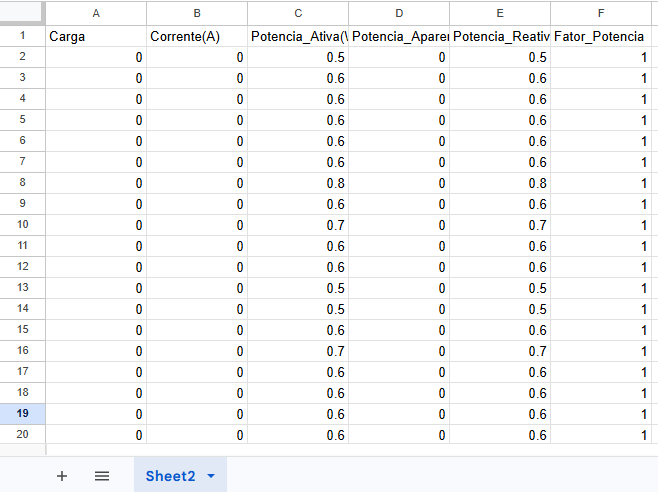
\includegraphics[width=\textwidth]{Figuras/Base de Dados - sheet2.png}
    \label{fig:planilha_dados_class}
    \fonte{\me{2026}}
\end{figure}

\begin{figure}[!htbp]
    \centering
    \caption{Visualização parcial da planilha de dados experimentais para o modelo de Regressão.}
    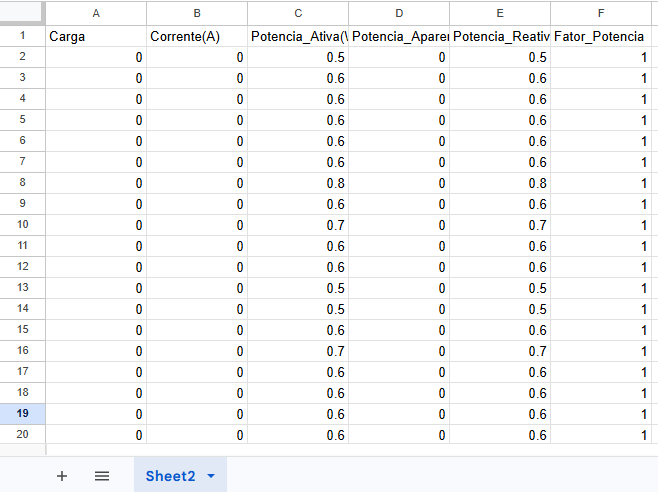
\includegraphics[width=\textwidth]{Figuras/Base de Dados - sheet2.png}
    \label{fig:planilha_dados_reg}
    \fonte{\me{2026}}
\end{figure}

As planilhas completas pode ser acessadas publicamente por meio do link:
\textbf{\url{https://drive.google.com/drive/folders/1i04sDnp_ZCUW4ox6y58tLU4OqA8bNqsv?usp=sharing}}


% ----------------------------------------------------------
% ----------------------------------------------------------
% APÊNDICE D - Código de integração entre o sensor PZEM-004T e o NodeMCU
% ----------------------------------------------------------
\chapter{Código de integração entre o sensor PZEM-004T e o Node MCU}
\label{apendice_integracao_PZEM_MQTT}

Código implementado em C++ para integração entre as medições do sensor PZEM-004T ao MQTT.

\begin{lstlisting}[language=C++, caption={Integração entre PZEM e MQTT.}, label=cod_integracao_PZEM_MQTT]
/*
===================================================================
Autor: Hirislayne Batista Ramos dos Santos
===================================================================
*/

#include <Arduino.h>
#include <PZEM004Tv30.h>
#include <ESP8266WiFi.h>
#include <PubSubClient.h>
#include <NTPClient.h>
#include <WiFiUdp.h>

#define BUILTIN_LED 2

// USANDO A SERIAL PADRÃO (GPIO1 E GPIO3) - NÃO USA SOFTWARE SERIAL!
PZEM004Tv30 pzem(Serial);  // PZEM nos pinos 1(TX) e 3(RX)

// Configurações de Rede e MQTT
const char* ssid = "NOME_RED_WIFI";
const char* password = "SENHA_REDE_WIFI";
const char* mqtt_server = "IP_REDE";
const char *mqtt_username = "tcc_hiris";
const char *mqtt_password = "tcc_hiris";

WiFiClient espClient;
PubSubClient client(espClient);
long lastMsg = 0;
char msg[200];

// Configuração do NTP
WiFiUDP ntpUDP;
NTPClient timeClient(ntpUDP, "a.st1.ntp.br", -3 * 3600, 60000); // -3 para Brasil

// Variáveis globais
float voltage = 0;
float current = 0;
float power = 0;
float energy = 0;
float frequency = 0;
float pf = 0;
float apparent = 0;
float reactive = 0;

void setup_wifi() {
  delay(10);
  // Sem debug, não podemos ver mensagens
  WiFi.begin(ssid, password);
  while (WiFi.status() != WL_CONNECTED) {
    delay(500);
    // Sem debug
  }
  randomSeed(micros());
}

void callback(char* topic, byte* payload, unsigned int length) {
  if ((char)payload[0] == '1') {
    digitalWrite(BUILTIN_LED, HIGH);
  } else {
    digitalWrite(BUILTIN_LED, LOW);
  }
}

void reconnect() {
  while (!client.connected()) {
    String clientId = "ESP8266Client-";
    clientId += String(random(0xffff), HEX);
    
    if (client.connect(clientId.c_str(), mqtt_username, mqtt_password)) {
      client.publish("status", "conectado!");
      client.subscribe("status");
    } else {
      delay(5000);
    }
  }
}

void setup() {
  // NÃO inicialize Serial.begin() - isso atrapalharia o PZEM!
  pinMode(BUILTIN_LED, OUTPUT);
  digitalWrite(BUILTIN_LED, LOW);
  
  setup_wifi();
  client.setServer(mqtt_server, 1883);
  client.setCallback(callback);
}

void loop() {
  if (!client.connected()) {
    reconnect();
  }
  client.loop();

  // Atualiza o horário
  timeClient.update();
  
  // Lê os dados do PZEM
  voltage = pzem.voltage();
  current = pzem.current();
  power = pzem.power();
  energy = pzem.energy();
  frequency = pzem.frequency();
  pf = pzem.pf();
  
  if(!isnan(voltage) && !isnan(current) && !isnan(power) && 
     !isnan(energy) && !isnan(frequency) && !isnan(pf)) {
    
    apparent = voltage * current;
    reactive = sqrt(abs(apparent * apparent - power * power));
    if (pf < 0) reactive = -reactive;
    
    long now = millis();
    if (now - lastMsg > 1000) {
      lastMsg = now;

      // Timestamp real
      unsigned long epochTime = timeClient.getEpochTime();
      String formattedTime = timeClient.getFormattedTime();
    
      // Criar um objeto JSON com todos os dados
      String payload = "{";
      payload += "\"tensao\":" + String(voltage) + ",";
      payload += "\"corrente\":" + String(current) + ",";
      payload += "\"potencia\":" + String(power) + ",";
      payload += "\"aparente\":" + String(apparent) + ",";
      payload += "\"reativa\":" + String(reactive) + ",";
      payload += "\"energia\":" + String(energy) + ",";
      payload += "\"frequencia\":" + String(frequency) + ",";
      payload += "\"fp\":" + String(pf) + ",";      
      payload += "\"timestamp\":" + String(epochTime) + ",";        // Unix timestamp
      payload += "\"hora\":\"" + formattedTime + "\",";             // Hora formatada
      payload += "\"timestamp_ms\":" + String(millis());            // ms desde boot
      payload += "}";
      
      // Publicar tudo em um único tópico
      client.publish("pzem/dados", payload.c_str());

      // Publicar os tópicos individuais
      snprintf(msg, 50, "%f", voltage);
      client.publish("tensao", msg);
      
      snprintf(msg, 50, "%f", current);
      client.publish("corrente", msg);
      
      snprintf(msg, 50, "%f", power);
      client.publish("potencia", msg);
      
      snprintf(msg, 50, "%f", apparent);
      client.publish("aparente", msg);
      
      snprintf(msg, 50, "%f", reactive);
      client.publish("reativa", msg);
      
      snprintf(msg, 50, "%f", energy);
      client.publish("energia", msg);
      
      snprintf(msg, 50, "%f", frequency);
      client.publish("frequencia", msg);
      
      snprintf(msg, 50, "%f", pf);
      client.publish("fp", msg);
      
    }
  }
  
  delay(1000);
}

\end{lstlisting}


% ----------------------------------------------------------
% ----------------------------------------------------------
% APÊNDICE E - Código da Análise da base de dados do PZEM
% ----------------------------------------------------------

\chapter{Código de Análise da Base de dados do PZEM}
\label{apendice_análise_PZEM}

Código implementado em Python utilizado na análise exploratória da base de dados coletada com o sensor PZEM-004T para ler o arquivo CSV com as medições e gerar um gráfico de dispersão que ilustra a relação entre corrente elétrica e potência ativa, destacando os agrupamentos correspondentes a cada tipo de carga.

\begin{lstlisting}[language=python, caption={Análise exploratória da base de dados do PZEM-004T.}, label=cod_analise_base_dados_pzem]
# ================================================================
# Autor: Hirislayne Batista Ramos dos Santos
# ================================================================

import pandas as pd
import matplotlib.pyplot as plt
import seaborn as sns
import numpy as np

df = pd.read_csv("/content/PZEM_dados - Sheet2.csv")

# Mapeamento das cargas
carga_map = {
    0: "Sem carga",
    1: "Capacitiva",
    2: "Indutiva",
    3: "Resistiva",
    4: "Motor",
    5: "Resistiva + Capacitiva",
    6: "Resistiva + Indutiva",
    7: "Capacitiva + Indutiva"
}

# Criar gráfico
plt.figure(figsize=(10, 6))

# Plotar cada carga
cargas = sorted(df['Carga'].unique())
cores = plt.cm.tab10(np.linspace(0, 1, len(cargas)))

for carga, cor in zip(cargas, cores):
    subset = df[df['Carga'] == carga]
    plt.scatter(subset['Corrente(A)'], 
               subset['Potencia_Ativa(W)'],
               color=cor, 
               label=carga_map[carga],
               alpha=0.6,
               s=25)

plt.xlabel('Corrente (A)', fontsize=12)
plt.ylabel('Potência Ativa (W)', fontsize=12)
plt.title('Corrente vs Potência Ativa por Tipo de Carga', fontsize=12)
plt.grid(True, linestyle='--', alpha=0.7)
plt.legend(title='Tipo de Carga', loc='upper left', fontsize=10)
plt.tight_layout()
plt.savefig('disp_corrente_potencia.png', dpi=300)
plt.show()

\end{lstlisting}

\end{apendicesenv}


% ----------------------------------------------------------
% ----------------------------------------------------------
% APÊNDICE F - Código da Análise descritiva da Base UCI
% ----------------------------------------------------------
% \chapter{Código de Análise da Base de dados da UCI}
% \label{apendice_análise_UCI}

% Código implementado em Python utilizado na análise exploratória da base UCI para realizar o pré-processamento dos dados, calcular o fator de potência e gerar as análises estatísticas e gráficos apresentados no Capítulo \ref{Resultados e Discussão}.

% \begin{lstlisting}[language=python, caption={Análise da Base de dados da UCI.}, label=cod_análise_base_dados_UCI]
% #  =============================================================
% #  Autor: Hirislayne Batista Ramos dos Santos
% #  =============================================================
% import pandas as pd
% import numpy as np
% import matplotlib.pyplot as plt
% import seaborn as sns
% import matplotlib.dates as mdates

% # ------- PRÉ-PROCESSAMENTO E ANÁLISE INICIAL ----
% # ---- Carregamento das Bases de dados - ano 2010 -------
% file_path = '/content/New_household_power_consumption_2010.csv'
% df= pd.read_csv(file_path, sep=',')
% df.head(5)
% df["Datetime"] = pd.to_datetime(df["Date"] + " " + df["Time"], format="mixed")
% df.set_index('Datetime', inplace=True)
% df.drop(['Date', 'Time'], axis=1, inplace=True)

% # ---- Informações gerais ----
% df.info()
% df.describe()

% # ----- Limpeza de valores ausentes por coluna ----
% print(df.isna().sum())
% df = df.dropna()
% print(df.isna().sum())

% # ---- Cálculo do FP -----
% df["Apparent_power"] = np.sqrt(df["Global_active_power"]**2 + df["Global_reactive_power"]**2)
% df["Power_factor"] = df["Global_active_power"] / df["Apparent_power"]
% df['Power_factor'] = df['Power_factor'].fillna(1.0) # Como podem haver divisões por zero (quando o consumo é 0), preenchemos com 1.0 (eficiência perfeita)


% # -------- ANÁLISES ----------
% # ------ Estatística do FP -----
% print("\nEstatísticas descritivas do Fator de Potência:")
% print(df["Power_factor"].describe())

% # ------Sazonalidade mensal do FP -----
% monthly_fp = df["Power_factor"].resample("M").mean()

% print("\n--- FP médio por mês ---")
% print(monthly_fp)

% # Criando a figura com tamanho adequado
% plt.figure(figsize=(12, 6))

% # Plot com marcadores para destacar os pontos
% plt.plot(monthly_fp.index, monthly_fp.values, 
%          marker='o',           # Adiciona marcadores circulares
%          linestyle='-',        # Linha sólida
%          linewidth=2,          # Espessura da linha
%          markersize=6,         # Tamanho dos marcadores
%          color='royalblue',    # Cor mais profissional
%          markerfacecolor='white',  # Marcador com centro branco
%          markeredgewidth=1.5,  # Borda do marcador
%          markeredgecolor='royalblue')  # Cor da borda

% # Configuração das grades (sua solicitação principal)
% plt.grid(True, which='major', linestyle='--', linewidth=0.5, alpha=0.7)
% plt.grid(True, which='minor', linestyle=':', linewidth=0.3, alpha=0.4)  # Grade menor opcional
% plt.minorticks_on()  # Ativa os ticks menores para a grade menor

% # Melhorando o eixo X (datas)
% plt.gca().xaxis.set_major_formatter(mdates.DateFormatter('%b/%Y'))  # Formato: Mês/Ano
% plt.gca().xaxis.set_major_locator(mdates.MonthLocator())  # Tick a cada mês

% # Título e labels com fontes maiores
% plt.title("Sazonalidade Mensal do Fator de Potência", pad=20)
% plt.xlabel("Mês/Ano")
% plt.ylabel("FP Médio")

% # Ajustes dos eixos
% plt.xticks(rotation=45, fontsize=10)
% plt.yticks(fontsize=10)

% # Adicionar linha de referência (limite mínimo ideal - exemplo)
% plt.axhline(y=0.92, color='red', linestyle='--', linewidth=1, alpha=0.7, label='Limite ideal (0.92)')

% # Adicionar valores nos pontos (opcional - comentado pois pode poluir)
% # for i, (x, y) in enumerate(zip(monthly_fp.index, monthly_fp.values)):
% #     plt.annotate(f'{y:.3f}', (x, y), textcoords="offset points", xytext=(0,10), ha='center', fontsize=8)

% # Limites do eixo Y (ajuste conforme seus dados)
% plt.ylim(0.85, 1.0)  # Ajuste baseado em valores típicos de FP

% # Legenda (se adicionar elementos como a linha de limite)
% plt.legend(loc='best', fontsize=10)

% # Layout ajustado
% plt.tight_layout()

% # Salvar a figura (opcional)
% # plt.savefig('sazonalidade_fp.png', dpi=300, bbox_inches='tight')

% plt.show()

% # ------- Correlação entre as variáveis --------
% cols = [
%     'Global_active_power', 'Global_reactive_power', 'Voltage',
%     'Global_intensity', 'Sub_metering_1', 'Sub_metering_2', 'Sub_metering_3',
%     "Apparent_power", "Power_factor"
% ]

% matriz_correlacao = df[cols].corr()

% plt.figure(figsize=(12, 8))
% sns.heatmap(matriz_correlacao, annot=True, cmap='RdBu', fmt=".2f", vmin=-1, vmax=1)
% plt.title("Mapa de Calor: Correlação entre Variáveis de Consumo")
% plt.show()

% # ------- Relações I, P, Q vs FP ----------
% plt.figure(figsize=(10, 6))
% sns.scatterplot(data=df.sample(min(2000, len(df))), x='Global_active_power', y='Power_factor', alpha=0.5, color="blue")
% plt.title('Relação Potência Ativa vs Fator de Potência')
% plt.xlabel('Potência Ativa (kW)')
% plt.ylabel('Fator de Potência')
% plt.grid(True, linestyle='--', alpha=0.7)
% plt.show()

% plt.figure(figsize=(10, 6))
% sns.scatterplot(data=df.sample(min(2000, len(df))), x='Global_intensity', y='Power_factor', alpha=0.5, color="orange")
% plt.title('Relação Corrente vs Fator de Potência')
% plt.xlabel('Corrente (A)')
% plt.ylabel('Fator de Potência')
% plt.grid(True, linestyle='--', alpha=0.7)
% plt.show()

% plt.figure(figsize=(10, 6))
% sns.scatterplot(data=df.sample(min(2000, len(df))), x='Global_reactive_power', y='Power_factor', alpha=0.5, color="green")
% plt.title('Relação Potência Reativa vs Fator de Potência')
% plt.xlabel('Potência Reativa (kVAr)')
% plt.ylabel('Fator de Potência')
% plt.grid(True, linestyle='--', alpha=0.7)
% plt.show()

% # ------- Periodo de ocorrencia dos menores FP ------------
% df['Hour'] = df.index.hour
% threshold_low = df["Power_factor"].quantile(0.01)
% lowest_fp = df[df["Power_factor"] <= threshold_low]

% print("Limite do 1% menor FP:", threshold_low)
% print("\nResumo estatístico dos menores FPs:")
% print(lowest_fp["Power_factor"].describe())

% print("\nDistribuição por hora (menores FPs):")
% print(lowest_fp["Hour"].value_counts().sort_index())

% # Gráfico melhorado
% plt.figure(figsize=(12, 6))

% # Histograma com bordas e cores
% counts, bins, patches = plt.hist(lowest_fp["Hour"], 
%                                  bins=24, 
%                                  range=(0, 24),
%                                  edgecolor='black', 
%                                  linewidth=1.2,
%                                  alpha=0.7,
%                                  color='steelblue')

% # Adicionar grades
% plt.grid(True, linestyle='--', alpha=0.6, axis='y')
% plt.grid(True, linestyle=':', alpha=0.3, axis='x', which='minor')

% # Configurações dos eixos
% plt.xticks(np.arange(0, 24, 2))
% plt.xticks(np.arange(0, 24, 1), minor=True)
% plt.xlabel("Hora do Dia")
% plt.ylabel("Frequência (Número de Ocorrências)")
% plt.title("Distribuição Horária dos 1% Menores Fatores de Potência", pad=15)

% # Adicionar linha de média
% plt.axhline(y=counts.mean(), color='red', linestyle='--', 
%             linewidth=1.5, alpha=0.7, label=f'Média: {counts.mean():.1f}')

% # Destacar pico
% max_idx = np.argmax(counts)
% plt.annotate(f'Pico: {int(counts[max_idx])}', 
%              xy=(bins[max_idx] + 0.5, counts[max_idx]), 
%              xytext=(bins[max_idx] + 2, counts[max_idx] + 2),
%              arrowprops=dict(arrowstyle='->', color='darkred'),
%              fontsize=10, fontweight='bold', color='darkred')

% # Legenda
% plt.legend(loc='upper right')

% # Ajustes finais
% plt.tight_layout()
% plt.show()

% */

% \end{lstlisting}
